\setchapterpreamble[u]{\margintoc}
\chapter{Conclusions and Future Work}\label{chapter-conclusions-and-future-work}

\epigraph{The woods are lovely, dark and deep,
But I have promises to keep,   
And miles to go before I sleep,   
And miles to go before I sleep.}{Robert Frost - 1874-1963}
% In the public domain according to https://poets.org/poem/stopping-woods-snowy-evening

Apps are a popular and relevant subset of all software, they run remotely on other people’s equipment where they are the primary owners of the data on their devices, and where the platform and pre-installed platform software determine various aspects of the data collection. The apps and the analytics libraries they use control what data is reported and when. 

When developers apply mobile analytics to find failures they are able to significantly improve the stability/reliability of their mobile app. When they stop paying attention and don't apply mobile analytics entropy returns eventually for a variety of reasons including new releases of the operating system, updates to third-party software used by the app, such as the Android System WebView, and flaws in ongoing software development and maintenance of the app. The developers do not need to address all the issues that are reported to effect material improvements (and indeed some issues are impractical for developers to fix in the time and resources they have available).

When developers choose to include in-app mobile analytics they generally prefer to use those mobile analytics as their primary source of information, even if the platform analytics also finds a common subset of the same failures. The meta-data collected and reported by the in-app mobile analytics combined with the availability of reports even at low usage volumes of the app are key drivers in this preference to use the in-app mobile analytics reporting. For two of the app-centric case studies the data collected by in-app mobile analytics \Glspl{sdk} was sufficient that they chose not to use in-app mobile analytics in their apps. Some projects choose to have several in-app \Glspl{sdk} embedded in their apps, often for distinct purposes.


\section{Summary of contributions}~\label{conclusions-summary-of-contributions}
If we revisit the research questions, first with the subsidiary questions, from ~\secref{rq-leads-to-six-perspectives}, we can get an overview of how the findings and discussion adress each of the,  The questions are reproduced here with a summary of the findings for each of the six perspectives: 

\newthought{1a. What do app developers say they do?} App developers have found mobile analytics useful. They vary in how they use them, some do so \emph{in extremis} so they can avert excessive failures, more generally they are used irregularly as and when they have the opportunity or need to do so. \myindex{Moonpig} used them on an ongoing, strategic basis and were rewarded by maintaining high reliability of their app with a correlation of business success as the business revenues grew and the company went Public (IPO'd). 

The human motivations that determine the use of mobile analytics are at least as interesting as the quantitative results of the effects of whatever use occurs. With the exception of the \myindex{Moonpig} development team, none of the teams used mobile analytics on an ongoing, proactive basis. 

\newthought{2a. What's possible in terms of improving their processes, their practices?}
As \myindex{Moonpig} and \myindex{Catrobat} project demonstrated it is viable to integrate mobile analytics into development practices. In the case of Moonpig, they added additional logging to the app (using \myindex{Firebase Analytics}) when they noticed or discovered new issues and/or areas of concern; they had developers on-point on-rotation to monitor and make initial decisions when fresh issues were observed in the mobile analytics, and they actively managed their fixes and releases using a composite of business and engineering risk assessments vs. benefits. While the Catrobat app-centric case study also highlighted benefits of analytics for improving processes and practices, it also identified the importance of projects having key personnel (e.g., product owners) who are responsible for maintaining these practices.

App developers are likely to materially improve the quality of their mobile apps when they actively engage with mobile analytics (whether in-app or platform generated), and even those who use in-app analytics extensively would benefit from actively checking the platform generated analytics as these capture issues and failures that in-app analytics do not.

Designing the apps so they emit pertinent information via mobile analytics (such as the approach used by \myindex{Moonpig}) may increase the value of the information being reported by the mobile analytics. One of the mini-experiments, details are in the appendices in \secref{app-mini-experiment-meta-dat-to-crash-logs}, corroborates a  similar approach to augment information reported by Crashlytics. 


\newthought{1b. What does their source code (and other available development artefacts) tell us about their use of mobile analytics?} 
Over 46\% of the active Android app codebases studied on GitHub simply initialised \myindex{Firebase Analytics} and did not use any other feature of the \Gls{sdk} (These projects were a tiny percentage of the opensource Android apps found on GitHub. All the commercial apps used mobile analytics extensively, while the \myindex{Catrobat} and \myindex{Kiwix} projects chose \emph{not} to use in-app mobile analytics. These results indicate commercial app developers rely on in-app mobile analytics including for detecting failures of their apps, in use. Services such as Google's \myindex{Android Vitals} provide, literally, a vital service for app developers, especially those who do not use in-app analytics.

All of the app-centric case studies recorded failures reported by mobile analytics in their issue-tracking system; none did so universally.

\newthought{2b. What's possible in terms of improving the product (and particularly the mobile app) through the application/use of mobile analytics?}


\newthought{1c. What do we learn about various current mobile analytics tools?}
There appears to be a general, perhaps misplaced, trust that the mobile analytics tools are accurate - both by the app developers and in the literature. Eighteen distinct flaws were found in the mobile analytics services, and there are probably many more flaws waiting to be discovered given the practical limitations placed by both industrial collaboration and the scope of a PhD. 


\newthought{2c. What improvements are possible for mobile analytics tools based on what was learned in the various case studies?}



The core question the research aims to consider is:
\begin{quote}
  \emph{How can applying analytics improve software development and software testing for mobile apps in practice?}~\href{overall-research-question}{Research Question, repeated here}\index{Research questions}.
\end{quote}






The field of mobile analytics evolved throughout the research period and it is likely to continue to evolve for years to come. The reporting and analysis appears to be fairly perfunctory and there may be significant scope to improve the analysis and reporting.




\clearpage
\section{Future Work}
%\subsection{Formulation of hypotheses for further study}
We have systematically explored the phenomena relating to the effect of mobile analytics on development processes and artefacts, see \secref{methodology-threats-to-validity-section}, here we use these findings to discuss areas for further study. The future work identified in this section incorporates future research work and areas for practitioners including app developers and tool developers.

\begin{figure}
    \centering
    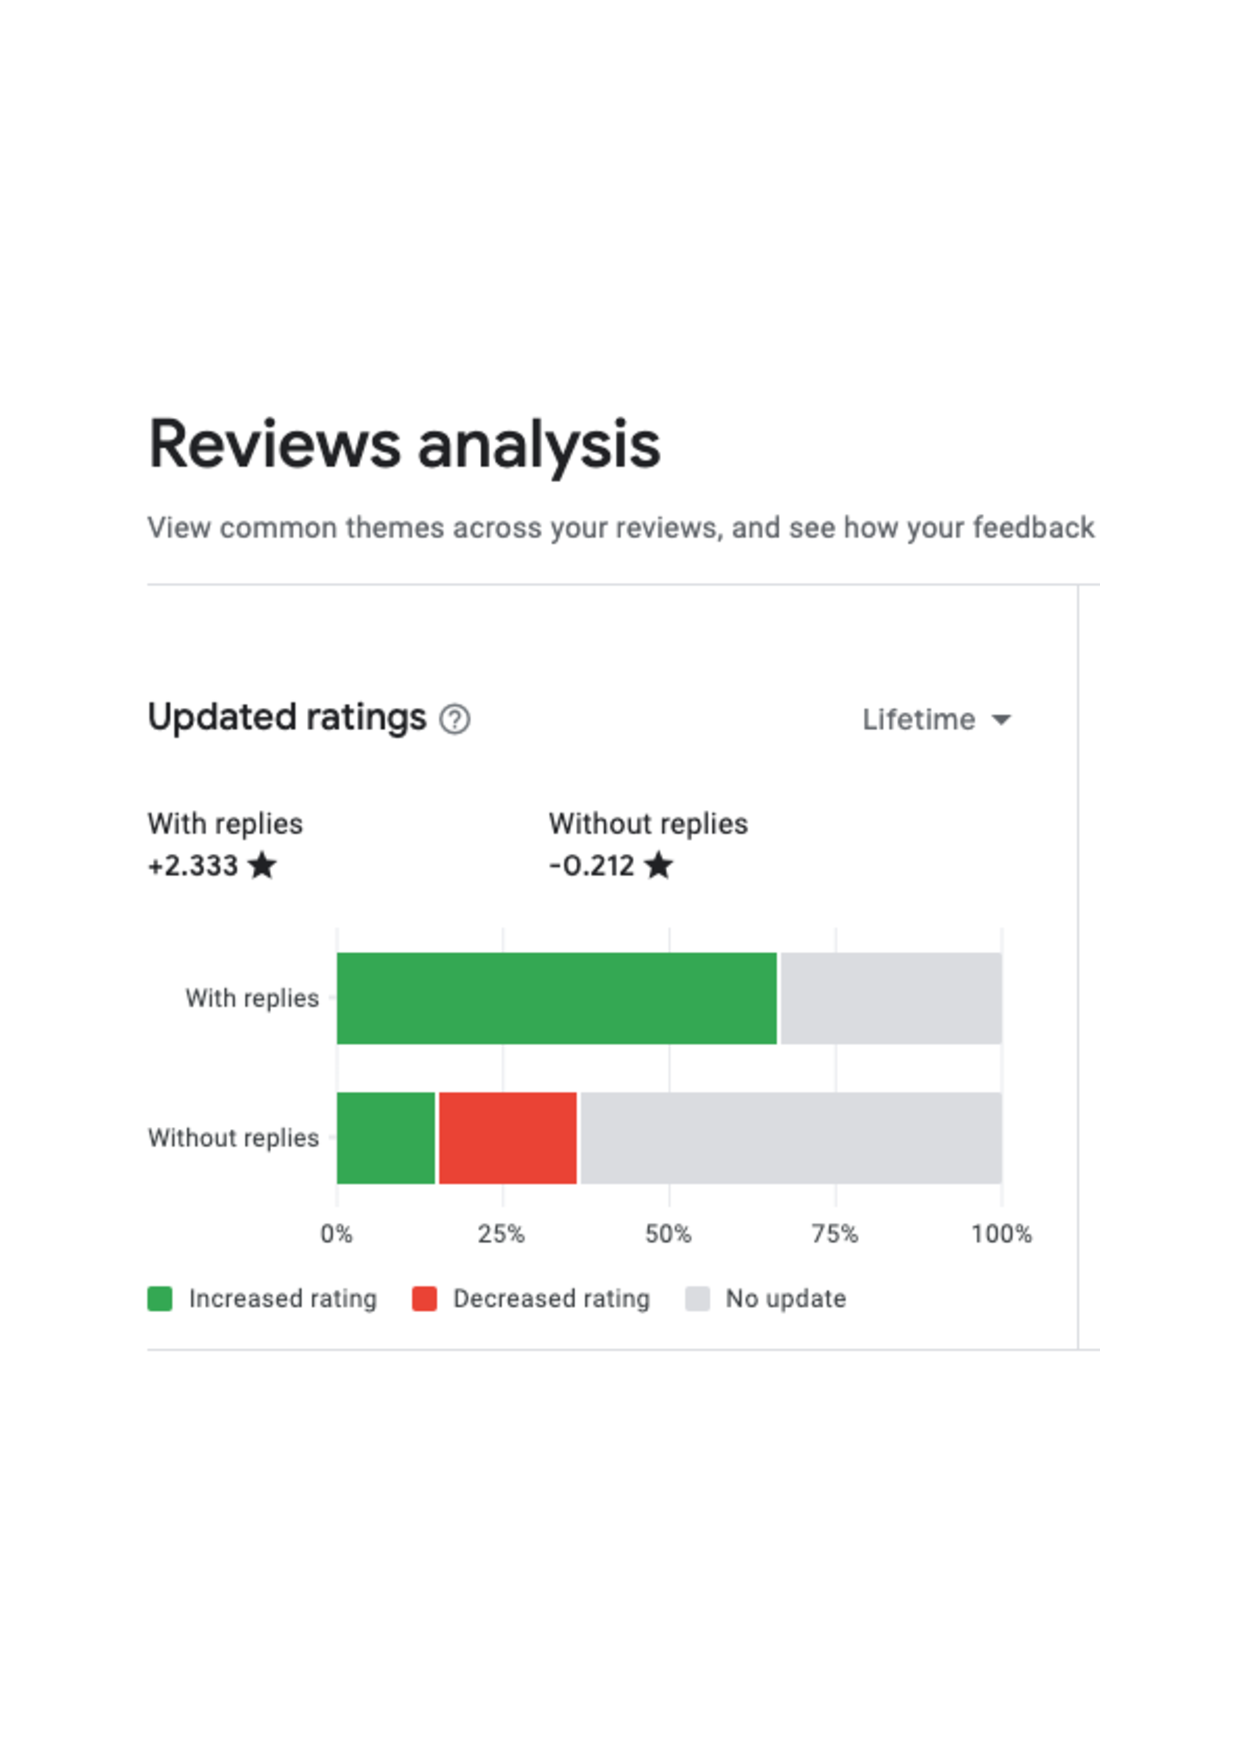
\includegraphics[width=\linewidth]{images/google-play-console/PhET-Review-Analysis-Screenshot-2022-09-07.pdf}
    \caption{Example of Review Analysis in Google Play Console for the Physics and Chemistry simulations app}
    \label{fig:PhET-Review-Analysis-Screenshot-2022-09-07}
\end{figure}

\begin{figure}
    \centering
    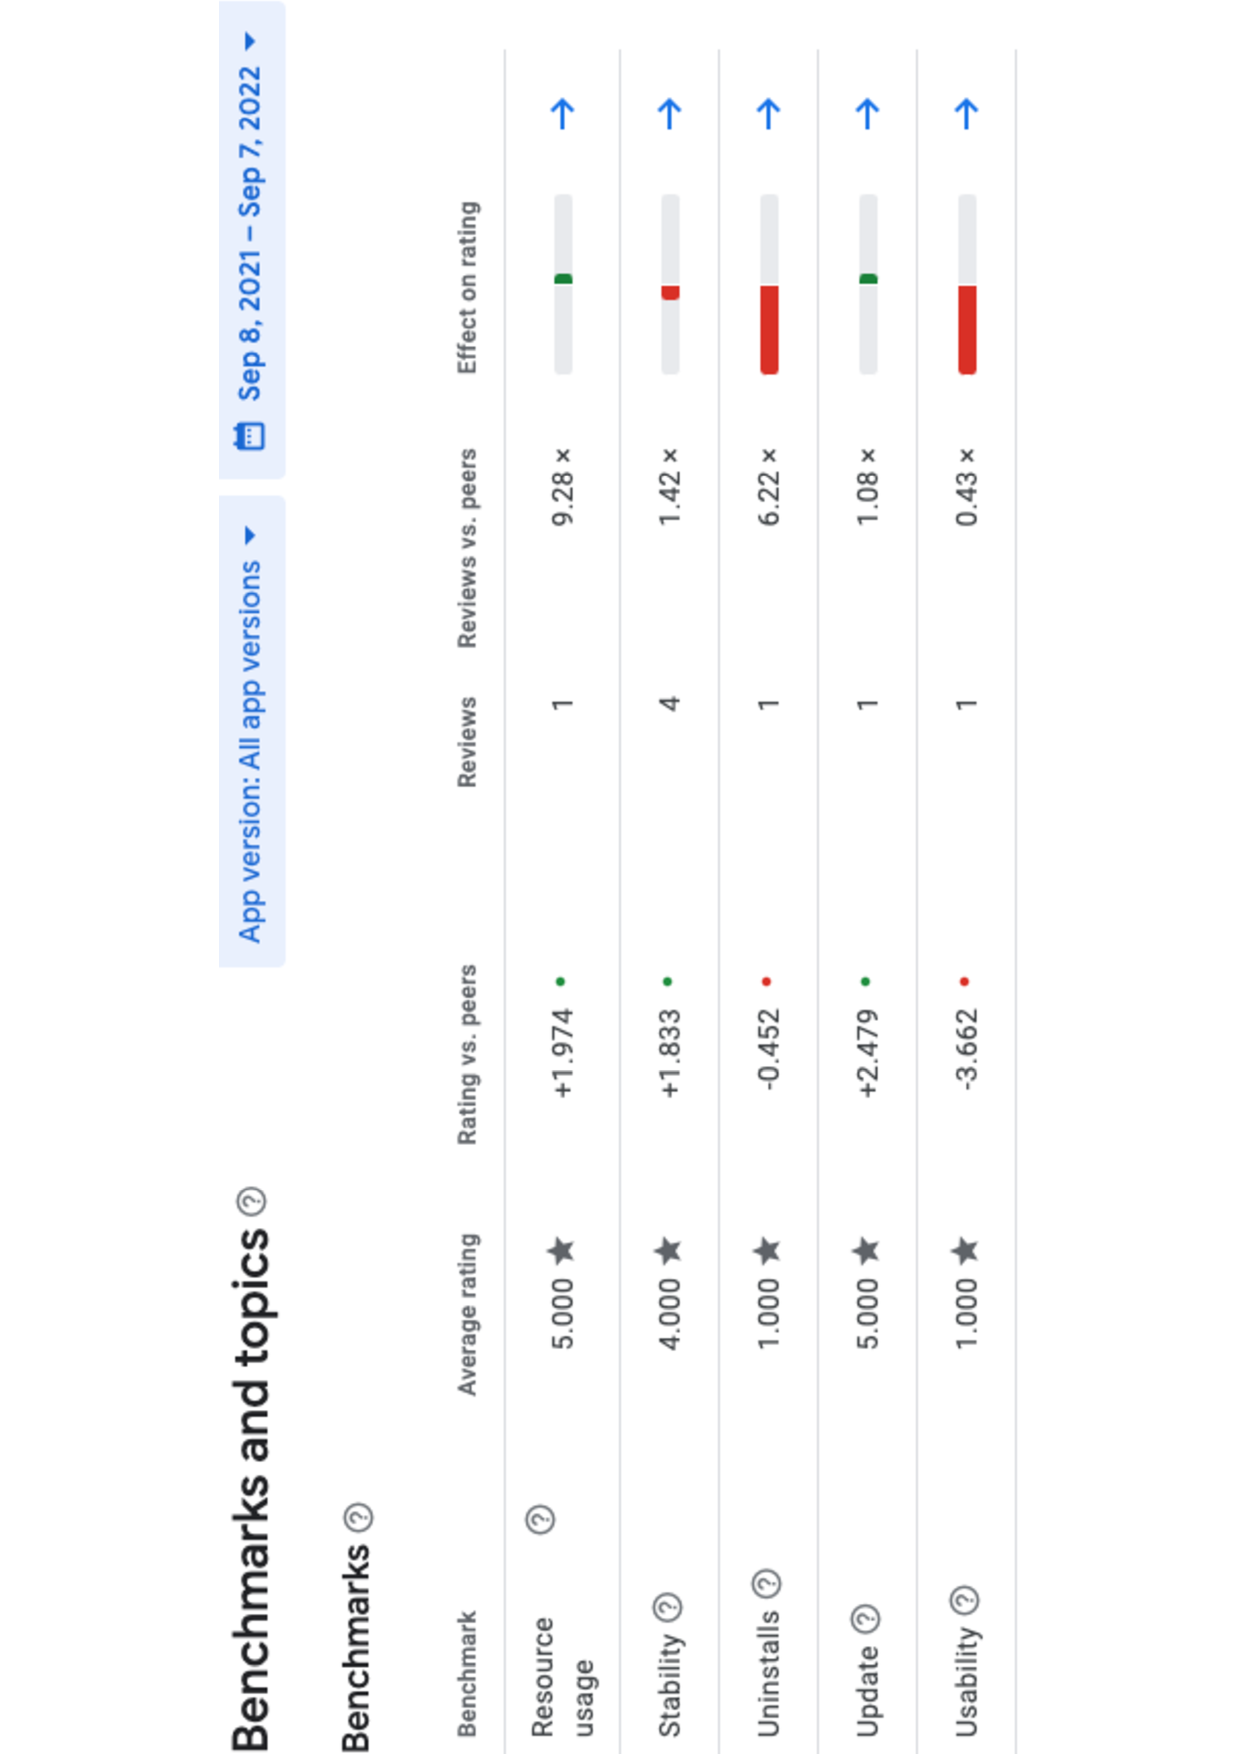
\includegraphics[width=\linewidth]{images/google-play-console/PhET-Review-Benchmarks-Screenshot-2022-09-07.pdf}
    \caption[Example for the \acrshort{phet} app of Benchmarks provided automatically by Google Play Console]{Example for the \Gls{phet} app of Benchmarks provided automatically by Google Play Console}
    \label{fig:PhET-Review-Benchmarks-Screenshot-2022-09-07}
\end{figure}

\subsection{Combining human- and mobile analytics feedback}~\label{fw-combining-reviews-and-mobile-analytics-topic}
In \secref{aiu-discussion-section} the concept of symbiotic information sources was discussed, for example to investigate any intersections and gaps between what users report in terms of bugs and crashes, \emph{etc.} and what mobile analytics reports. Android app developers have good access to both platform analytics, via \myindex{Android Vitals}, and various online Review Analysis tools, illustrated in Figures \ref{fig:PhET-Review-Analysis-Screenshot-2022-09-07} and \ref{fig:PhET-Review-Benchmarks-Screenshot-2022-09-07}, to the best of my knowledge there has not been material research either into the Review Analysis tools, nor into any symbiosis between the reviews, review analysis, or mobile analytics. Such research may provide insights into the review analysis (which may have its own flaws and characteristics) and the extent to which mobile analytics and reviews provide actionable information to developers, \emph{etc.}

\newthought{Symbiotic information sources: }
Development teams can use both mobile analytics and user feedback where they complement each other. There was only one example, from Moonpig in \secref{aiu-interventions-theme} where the two sources were combined and contrasted, there may have been other instances but they were not captured in the research. 

An useful example from grey literature of how the two sources of information have helped developers is described in \sidecite{sunderland2019_the_one_star_android_review}. The meta-information Google Android collected when the user wrote the review indicated the user's device had a low screen resolution. The developer was able to recreate an Android virtual device with the same screen dimensions and reproduce the bug. They then added a specific screen layout suitable for this and other low screen resolution devices.

Existing research by Microsoft in software analytics found that Data/Metrics and Customer input were both deemed important by both managers and developers which indicate the potential of combining both these sources of information.~\sidecite[][p. 989]{buse2012_information_needs_for_software_development_analytics}

Symbiotic information sources would be a fruitful area of future work, and is discussed in \secref{fw-combining-reviews-and-mobile-analytics-topic}.

The overall development process for mobile apps includes both the release and operational stages of a software lifecycle. Recent research aims to determine whether releases are good, bad, or neutral. One of their key observations is ``Android developers need to pay attention to the quality of their app next release''~\sidecite[][p. 31]{saidani2022_tracking_bad_updates_in_mobile_apps_a_search_based_approach}. They plan to extend their \uppercase{App-Tracker} software tool so it can be integrated into the development pipeline for Android apps which sounds promising, especially if the underlying software could also use mobile analytics data as part of the scoring of a potential release.


\subsection{Investigation of additional app ecosystems}~\label{fw-investigate-additional-ecosystems}
If the mobile app ecosystem influences other ecosystems such as desktop app ecosystems\index{Desktop app ecosystem}, as claimed in the opening section of \secref{chapter-related-work}, perhaps this research will also apply to those app ecosystems, albeit there are likely to be many distinctions as each ecosystem is distinct and unique.  What are the engineering challenges and realities in those app ecosystems, what sort of analytics do those platforms provide? and what do the apps use? To what extent can the app developers rely on analytics to learn of instabilities or failures in their apps, and can they apply similar techniques to those described in this research? 

Closer to home, there has been little study of mobile analytics in regional app stores, such as those in China~\sidecite{wang2018_beyond_google_play}.


\subsection{Establishing transparency and trust in mobile analytics}~\label{fw-establishing-transparency-and-trust-in-mobile-analytics}
There are existing fragments that provide elements of transparency and trust in mobile analytics tools and services, for example, opensource \Glspl{sdk} and servers, the \myindex{CrashScope} initiative, Google and many others who are involved in the \href{https://www.openmined.org/}{OpenMined}\index{OpenMined} initiative~\sidecite{track2021_openmined_case_study} % and https://developers.googleblog.com/2021/01/how-were-helping-developers-with-differential-privacy.html
where there are tools and the willingness to establish trust in the design \emph{and} implementation of data-based research and analysis. This is an area where the combination of industry support and academic research may bear much fruit. 

The following list of considerations have been highlighted during the research as being relevant to addressing concerns of trust and transparency when using mobile analytics. Further investigation is required to get a better understanding of how they impact mobile app development practice and the quality of the apps produced.

\begin{itemize}
    \item Privacy: protecting the privacy of the end users. 
    \item Ownership and uses: especially in terms of who owns the data and who gets to use it?:
    \item Stewardship: Impact(s) of having access to sensitive and valuable data.  
    \item Trust: [Over] trust in decisions made by technology, see \secref{discussion-human-behaviours-around-automation-topic}.
\end{itemize}


\subsection{Operational considerations when using Mobile Analytics}~\label{fw-operational-considerations-topic}
In addition to research into establishing transparency and trust there are various operational considerations that warrant further research. These include: 

\begin{itemize}
    \item Sufficiency: in the context of collecting sufficient to enable us to achieve our objectives of improving our software and our processes.    
    \item Costs: financial, data, privacy, performance, bloat. These are closely aligned to performance aspects.
    \item Performance: which includes runtime overhead, transmission overhead, latency and scalability.
\end{itemize}


\section{Final thoughts}~\label{final-thoughts-to-the-thesis}
Before the research was undertaken we didn't understand these themes. We now have a better understanding of how .... The research also provides evidence about the utility and effectiveness about using mobile analytics to improve the quality of mobile apps in a real world context. It is hoped this encourages and inspires greater use of ma and further research into this important area.
